\chapter*{Chapter 7: Diễn giải mạng nơ-ron}

Chương này tập trung vào các phương pháp diễn giải cho mạng nơ-ron. Các phương pháp trực quan hóa đặc trưng và khái niệm (concepts) được học bởi một mạng nơ-ron, giải thích các dự đoán và đơn giản hóa mạng nơ-ron.

Học sâu (deep learning) đã trở nên cực kỳ thành công, đặc biệt trong các tác vụ liên quan đến xử lý hình ảnh và văn bản như phân loại ảnh (image classification) và dịch máy (translation). Câu chuyện thành công của các mạng nơ-ron sâu bắt đầu từ năm 2012, khi mà cuộc thi phân loại ảnh trên tập dữ liệu ImageNet có nhà vô địch sử dụng phương pháp học sâu. Từ đó tới nay, ta đã chứng kiến sự bùng nổ mạnh mẽ của các cấu trúc mạng nơ-ron sâu, với xu thế tăng dần về độ sâu và số lượng các trọng số của mạng nơ-ron.

Để tạo ra các dự đoán, dữ liệu được đưa qua rất nhiều tầng hay lớp (layer) và nhân với các trọng số đã được học cùng với các phép biến đổi phi tuyến. Một dự đoán đơn lẻ có thể liên quan đến hàng triệu phép tính toán phụ thuộc vào cấu trúc của mạng nơ-ron. Rõ ràng ta không thể theo dõi từng ánh xạ và các biến đổi diễn ra trong mạng nơ-ron. Ta có thể xem xét hàng triệu trọng số tương tác với nhau theo các cách phức tạp để sáng tỏ cách mà một dự đoán được tạo ra. Để diễn giải cách thức hoạt động và các dự đoán của các mạng nơ-ron, ta cần các phương pháp diễn giải cụ thể. Bạn cần có kiến thức về học sâu và mạng nơ-ron tích chập trước khi đi vào chương này.

Ta chắc chắn có thể sử dụng các phương pháp phân tích kiểu mẫu (model-agnostic), ví dụ như LIME hoặc PDP (Partial Dependence Plot), nhưng có hai lý do chính tại sao ta lại cần những phương pháp khác, mà đặc biệt dùng để phân tích các mạng nơ-ron. Thứ nhất, mạng nơ-ron học các đặc trưng và khái niệm ở trong các lớp ẩn (hidden layers) và ta cần các công cụ đặc biệt để có thể khai phá chúng. Thứ hai, gradient có thể được dùng để tạo ra các phương pháp mà có độ phức tạp về tính toán thấp hơn so với các công cụ kiểu mẫu (phân tích mạng từ bên ngoài). Hầu hết các phương pháp trong cuốn sách này nhằm giải thích các mô hình xây dựng từ dữ liệu dạng bảng (tabular). Ảnh và văn bản cần các phương pháp khác.


\section{Các đặc trưng được học}

Mạng thần kinh tích chập học các đặc trưng trừu tượng và khái niệm trừu tượng từ các điểm ảnh của hình ảnh gốc. Trực quan hóa đặc trưng biểu diễn các đặc trưng đã được học thông qua việc cực đại hóa kích hoạt (activation maximization). Phân tách mạng \href{https://christophm.github.io/interpretable-ml-book/cnn-features.html#network-dissection}{Network Dissection} gán nhãn các đặc trưng của mạng thần kinh (ví dụ như các kênh) với các khái niệm của con người.

Các mạng nơ-ron sâu học các đặc trưng cấp cao (high-level features) trong các lớp ẩn của mạng. Đây là một trong những thế mạnh to lớn nhất và điều này làm giảm thiểu sự cần thiết của các kỹ thuật đặc trưng (feature engineering). Giả sử bạn muốn xây dựng một bộ phân loại hình ảnh với Support Vector Machine (SVM). Ma trận các điểm ảnh thô không phải là đầu vào tốt nhất cho việc huấn luyện mô hình SVM của chúng ta, nên ta cần tạo ra các đặc trưng mới dựa trên màu sắc, miền tần số (frequency domain), phát hiện cạnh, vân vân. Với mạng thần kinh tích chập, hình ảnh được đưa vào trong mạng là các mẫu thô (điểm ảnh), sau đó mạng biến đổi hình ảnh đầu vào nhiều lần. Đầu tiên, hình ảnh đi qua nhiều lớp tích chập. Trong những lớp tích chập này, mạng học những đặc trưng mới và ngày càng tăng độ phức tạp trong các lớp đó. Sau đó những thông tin của hình đã được ảnh biến đổi đi qua các lớp liên kết đầy đủ (fully connected) và trả về kết quả.

\newpage

\begin{figure*}[h!]
	\centering
	\includegraphics[scale=0.45]{images/cnn-features.png}
	\label{fig:7_1}
	\caption{Các đặc trưng học được bởi mạng thần kinh tích chập (Inception V1) được huấn luyện trên tập dữ liệu ImageNet. Các đặc trưng được sắp xếp thứ tự từ những đặc trưng đơn giản trong các lớp tích chập thấp hơn (trái) đến trừu tượng hơn trong các lớp tích chập cao hơn (phải). Hình ảnh từ Olah, et al. 2017 (CC-BY 4.0) \href{https://distill.pub/2017/feature-visualization/appendix/}{xem thêm}.}
\end{figure*}

- Các đặc trưng của những lớp tích chập đầu tiên là cạnh và một số kết cấu đơn giản. 

- Các đặc trưng của các lớp tích chập sau đó là các họa tiết (patterns or textures) và kết cấu phức tạp hơn một chút.

- Các đặc trưng của các lớp tích chập cuối là vật thể hoặc một phần của vật thể.

- Các lớp kết nối đầy đủ liên kết các kích hoạt từ các đặc trưng bậc cao đến các lớp độc lập để tạo ra dự đoán cuối cùng.

Vậy là ta đã nắm một số khái niệm để hình dung về các đặc trưng được học bởi mạng nơ-ron, vậy bằng cách nào chúng ta có thể biểu diễn chúng một cách trực quan?

\subsection{Trực quan hóa đặc trưng}

Cách tiếp cận việc tạo ra các đặc trưng một cách minh bạch như thế này được gọi là trực quan hóa đặc trưng (feature visualization). Trực quan hóa đặc trưng cho một thành phần của mạng thần kinh là việc tìm ra đầu vào mà sẽ làm tối đa hóa kích hoạt của thành phần đó.

“Thành phần” nghĩa là nơ-ron đơn lẻ, hoặc các kênh (hay còn gọi là bản đồ đặc trưng (feature maps)), hay toàn bộ lớp hoặc xác suất trả về bởi lớp cuối cùng trong bộ phân loại (hoặc tương đương với nơ-ron pre-softmax mà ta đang quan tâm). Các nơ-ron độc lập là thành phần nguyên tử của mạng, nên chúng ta sẽ lấy được hầu hết thông tin bằng cách tạo các trực quan hóa đặc trưng cho mỗi nơ-ron. Nhưng có một vấn đề: Các mạng nơ-ron thường chứa hàng triệu các nơ-ron. Nếu nhìn vào mỗi trực quan hóa của từng đặc trưng thì sẽ rất tốn thời gian. Các kênh (thường được gọi là các bản đồ kích hoạt - activation maps) là một lựa chọn không tồi cho việc trực quan hóa đặc trưng. Chúng ta có thể đi một bước xa hơn và trực quan hóa cả một lớp tích chập hoàn toàn (entire convolutional layer). Việc coi các lớp như là một thành phần được sử dụng trong DeepDream của Google, khi ta liên tục lặp đi lặp lại các trực quan hóa đặc trưng của một lớp vào hình ảnh gốc, kết quả cuối cùng là một phiên bản như mơ ước của đầu vào (ảnh mà sẽ làm cực đại hóa tất cả các thành phần của mạng nơ-ron).

\begin{figure*}[h!]
	\centering
	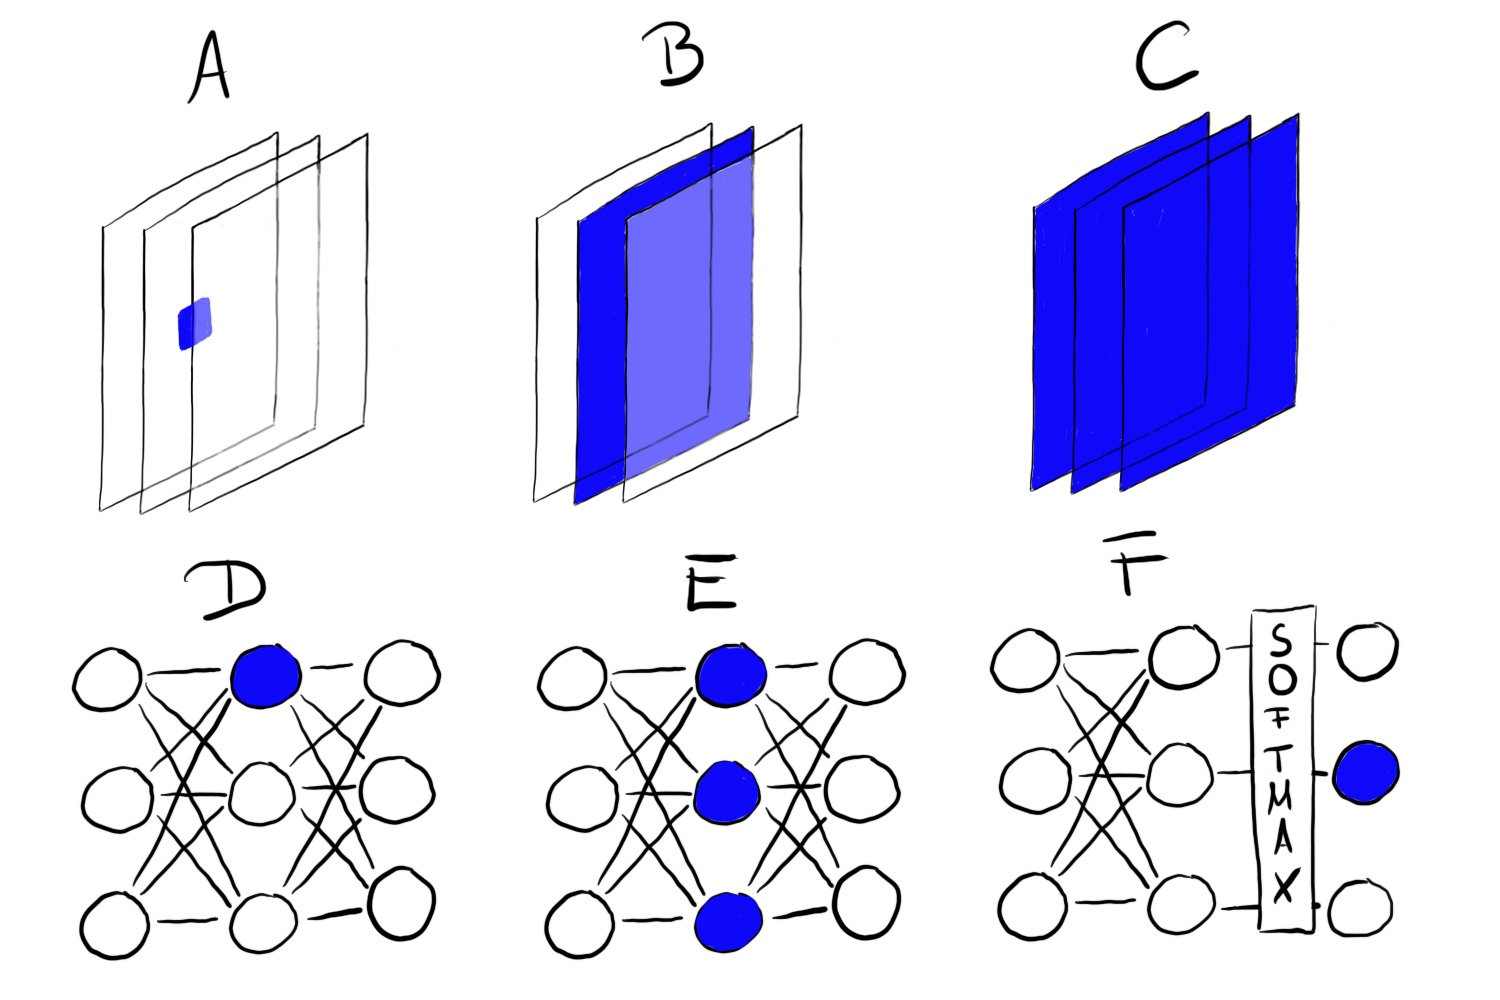
\includegraphics[scale=0.3]{images/units.jpg}
	\label{fig:7_2}
	\caption{Trực quan hóa có thể tạo ra từ các thành phần khác nhau. A) Nơ-ron tích chập, B) Kênh tích chập, C) Lớp tích chập, D) Nơ-ron, E) Lớp ẩn, F) Nơ-ron xác suất phân loại lớp (hoặc tương đương với nơ-ron pre-softmax).}
\end{figure*}

\subsubsection{Trực quan hóa đặc trưng thông qua tối ưu hóa}

Trong các thuật ngữ toán học, trực quan hóa là một vấn đề tối ưu. Chúng ta giả sử rằng các trọng số của mạng là được cố định, có nghĩa rằng một mạng được huấn luyện. Chúng ta tìm kiếm một hình ảnh mới mà tối đa hóa (trung bình) kích hoạt một thành phần, ở đây là một nơ-ron đơn:

\[img^*=\arg\max_{img}h_{n,x,y,z}(img)\]

Hàm h là hàm kích hoạt của một nơ-ron, img là đầu vào của một mạng (thường là hình ảnh), x và y mô tả không gian vị trí của nơ-ron, n là chỉ số lớp và z là chỉ số kênh. Đối với kích hoạt trung bình của toàn bộ kênh z trong lớp n chúng ta tối đa hóa:

\[img^*=\arg\max_{img}\sum_{x,y}h_{n,x,y,z}(img)\]

Trong công thức này, tất cả nơ-ron trong kênh z là có trọng số như nhau. Ngoài ra, ta cũng có thể tối đa hóa các hướng ngẫu nhiên, nghĩa là  các nơ-trong sẽ được nhân bởi các tham số khác nhau, bao gồm cả các chiều âm. Trong trường hợp này, chúng ta nghiên cứu cách mà các nơ-ron tương tác với nhau trong kênh. Thay vì tối đa hóa kích hoạt, ta cũng có thể tối thiểu hóa các giá trị này (tương đương với tối đa hóa theo chiều âm). Một điều rất thú vị, khi ta tối đa hóa theo chiều âm, ta tạo sẽ thu về đặc trưng rất khác biệt cho cùng thành phần:

\begin{figure*}[h!]
	\centering
	\includegraphics[scale=1.3]{images/a484.png}
	\label{fig:7_3}
	\caption{Kích hoạt dương (trái) và âm (phải) của Inception V1 nơ-ron 484 từ lớp mix4d pre relu. Trong khi nơ-ron là được kích hoạt (activation) mạnh nhất bởi các bánh xe, thì có một thứ gì đó trông giống như có mắt sinh ra từ kích hoạt âm (\href{https://colab.research.google.com/github/tensorflow/lucid/blob/master/notebooks/feature-visualization/negative_neurons.ipynb}{code}).}
\end{figure*}

Chúng ta có thể giải quyết bài toán tối ưu này theo các cách khác nhau. Đầu tiên, tại sao chúng ta lại sinh ra các hình ảnh mới? Chúng ta có thể đơn giản hóa bằng cách tìm kiếm trên các ảnh trong tập huấn luyện và lựa chọn những bức ảnh làm cực đại kích hoạt. Đây là một cách tiếp cận hợp lý, nhưng sử dụng dữ liệu huấn luyện có một vấn đề là các thành phần trong các hình ảnh có thể bị tương quan và chúng ta không thể nhìn thấy những gì mà mạng nơ-ron thực sự nhìn thấy. Nếu các hình ảnh trên sinh ra một kích hoạt (activation) cao trên kênh hiện tại và ảnh đó thể hiện một con chó và một quả bóng tennis, chúng ta không biết cái nào mà mạng nơ-ron đang quan tâm, là con chó, là quả bóng tennis hay là có thể cả hai.

Một cách tiếp cận khác là tạo ra các hình ảnh mới, bắt đầu từ các nhiễu ngẫu nhiên (random noise). Để thu được các hình ảnh trực quan có nghĩa, ta chấp nhận những ràng buộc trong hình ảnh, ví dụ chỉ có các thay đổi nhỏ là được cho phép. Để giảm thiểu nhiễu trong trực quan hóa đặc trưng, ta có thể áp dụng các rung động (jittering), xoay hoặc thay đổi tỷ lệ hình ảnh trước bước tối ưu hóa. Các phương pháp khác sẽ dựa trên việc diều chuẩn (regularization) bao gồm trừng phạt tần suất (ví dụ giảm phương sai của các điểm ảnh lân cận) hoặc sinh ra các hình ảnh với xác suất tiên nghiệm đã học trước đó (learned priors), ví dụ với các mạng GANs (Generative adversarial networks) hoặc mạng giảm nhiễu autoencoders (denoising autoencoders).

\begin{figure*}[h!]
	\centering
	\includegraphics[scale=0.5]{images/activation-optim.png}
	\label{fig:7_4}
	\caption{Tối ưu hóa lặp đi lặp lại từ các hình ảnh ngẫu nhiên để tối đa hóa kích hoạt.}
\end{figure*}

Nếu bạn muốn tìm hiểu sâu hơn về trực quan hóa đặc trưng, hãy xem qua trang tạp chí distill.pub, đặc biệt các trực quan hóa đặc trưng được đăng bởi Olah et al. Cuốn sách này có sử dụng nhiều hình ảnh cũng như các khối (building blocks) liên quan đến tính khả năng diễn giải.

\subsubsection{Liên hệ tới các ví dụ của học đối kháng  (Adversarial Examples)}

Có một liên kết giữa trực quan hóa đặc trưng và các ví dụ đối kháng: Cả hai kỹ thuật đều tối đa hóa kích hoạt của thành phần mạng nơ-ron. Với các ví dụ đối kháng, chúng ta tìm kiếm các kích hoạt tối đa của nơ-ron cho các lớp phản nghich (= lớp không chính xác). Một khác biệt là với hình ảnh chúng ta bắt đầu: Đối với các ví dụ đối kháng, nó là hình ảnh mà chúng ta muốn sinh ra hình ảnh đối kháng. Đối với trực quan hóa đặc trưng nó là các nhiễu ngẫu nhiên, và phụ thuộc vào phương pháp tiếp cận.

\subsubsection{Dữ liệu văn bản và bảng}

Các nghiên cứu hiện nay đang tập trung vào trực quan hóa đặc trưng mạng nơ-ron tích chập trong bài toán nhận diện hình ảnh (image recognition). Về mặt kỹ thuật, không có điều gì ngăn ta tìm đầu vào mà tối đa kích hoạt của một nơ-ron của mạng nơ-ron liên kết đầy đủ cho dữ liệu bảng hoặc một mạng nơ-ron hồi tiếp (recurrent neural network) cho dữ liệu văn bản. Bạn có thể không thể gọi nó là trực quan hóa đặc trưng nữa, vì các đặc trưng sẽ là dữ liệu đầu vào dạng bảng hoặc văn bản. Ví dụ đối với bài toán với dự đoán tín dụng mặc định, các đầu vào có thể là số lượng các tín dụng trước đó, số lượng các hợp đồng di động, địa chỉ và hàng tá các đặc trưng khác. Các đặc trưng được học của một nơ-ron sẽ là sự kết hợp nhất định của hàng tá các đặc trưng này. Còn đối với mạng nơ-ron hồi tiếp, nó có chút dễ dàng hơn để trực quan những gì mạng nơ-ron học được: Karpatht et. al (2015) đã chỉ ra rằng mạng nơ-ron hồi tiếp thực sự có các nơ-ron mà học những đặc trưng khả diễn giải. Chúng huấn luyện một mô hình dưới cấp độ các ký tự, nó dự đoán những ký tự tiếp theo trong chuỗi từ những ký tự trước đó. Một khi dấu mở ngoặc “(” xuất hiện, một trong những nơ-ron đạt kích hoạt cao, và nơ-ron bị vô hiệu hóa khi một dấu đóng ngoặc ")" xuất hiện. Các nơ-ron khác
được kích hoạt ở cuối dòng. Một số nơ-ron bị kích thích bở các đường dẫn (URLs). Sự khác biệt so với trực quan hóa đặc trưng cho CNNs đó là các mẫu dữ liệu không được tìm thấy thông qua tối ưu, mà thông qua việc nghiên cứu các kích hoạt trong dữ liệu huấn luyện.
Một số hình ảnh có nội dung thể hiện trông giống như mõm chó hoặc tòa nhà. Nhưng làm thế nào để chúng ta có thể chắc chắn được? Phương pháp phân tách mạng (Network Dissection) liên kết các khái niệm của con người với các thành phần nơ-ron độc lập. Cảnh báo trước: Phương pháp phân tách mạng (Network Dissection) yêu cầu thêm dữ liệu bổ sung mà trước đó ta cần gán nhãn với các khái niệm của con người.

\subsection{Phân tách mạng (Network Dissection)}

Phân tách mạng được phát minh bởi Bau \& Zhou et al. (2017) phương pháp này lượng khả năng diễn giải một thành phần của một mạng nơ-ron tích chập. Phương pháp này gán nhãn cho các kênh của CNNs với các khái niệm của con người (đối tượng, bộ phận, kết cấu, màu sắc,…).

Các kênh của mạng nơ-ron tích chập học các đặc trưng mới, như chúng ta đã thấy trong chương này về phần  \href{https://christophm.github.io/interpretable-ml-book/cnn-features.html#feature-visualization}{trực quan hóa đặc trưng}. Nhưng những trực quan hóa này không chứng minh được rằng một thành phần đã học một khái niệm nhất định hay không? Chúng ta cũng không đo lường được hiệu quả hoạt động trong việc nhận biết vật thể của một thành phần là tốt như thế nào. Trước khi chúng ta đi vào chi tiết về phân tách mạng, trước hết cần đề cập tới những giả thiết của phương pháp này. Những giả thuyết này là: Các thành phần của mạng nơ-ron (như là các kênh tích chập) học những khái niệm riêng rẽ với nhau (disentangled concepts). 

\textbf{Các đặc trưng riêng rẽ}

Liệu mạng nơ-ron học các đặc trưng riêng rẽ (disentangled features)? Đặc trưng riêng rẽ nghĩa là các thành phần mạng riêng lẻ phát hiện các khái niệm cụ thể khác nhau. Ví dụ, kênh tích chập 394 có thể phát hiện tòa nhà chọc trời, kênh 121 là mõm chó, kênh 12 là sọc ở góc 30 độ … Đối lập với mạng tách bạch (Disentangled network) là một mạng không tách bạch (Entangled network). Trong mạng hoàn toàn phi tách bạch, ví dụ, không có bất cứ kênh đơn lẻ nào gắn với mõm chó. Tất cả các kênh đều đóng góp để nhận diện mõm chó.

Các tính năng tách bạch hàm ý rằng mạng có tính khả diễn giải cao. Chúng ta giả sử rằng có một mạng với các thành phần hoàn toàn tách bạch đã được gán nhãn với các khái niệm đã biết. Điều này sẽ giúp việc giám sát quy trình tạo ra các quyết định của mạng trở nên dễ dàng hơn. Ví dụ, chúng ta phân tích cách mà mạng nơ-ron phân loại chó husky với sói. Đầu tiên chúng ta xác định các đặc trưng của chó husky. Khi ta đưa vào một ảnh của chó husky, ta có thể kiểm tra liệu kết quả có phụ thuộc vào thành phần ``mõm chó'', ``lông mịn'' và ``tuyết'' từ các lớp phía trước hay không. Nếu có, chúng ta biết rằng nó sẽ đang phân loại chính xác. Trong một mạng tách bạch (disentangled),, chúng ta có thể chỉ ra các mối tương quan phi nhân quả. Chúng ta có thể tự động liệt kê tất cả các thành phần kích hoạt và khái niệm của chúng để giải thích một dự đoán độc lập. Hơn nữa, ta có thể dễ dàng phát hiện sai lệch trong mạng nơ-ron. Ví dụ, mạng có học đặc trưng “da trắng” để dự đoán lương của một người hay không)?

Thực tế: Mạng nơ-ron tích chập không phải là tách bạch. Chúng ta sẽ xem xét chi tiết hơn thuật toán để tìm ra như thế nào là một mạng nơ-ron khả diễn giải.

\subsubsection{Thuật toán phân tách mạng}

Phân tách mạng có ba bước:

\begin{enumerate}
  \item Lấy vào hình ảnh với nhãn đã được con người gán với khái niệm trực quan.
  \item Đo đạc các kích hoạt của kênh cho những hình ảnh này.
  \item Định lượng sự tương quan giữa kích hoạt và các khái niệm đã được dán nhãn
\end{enumerate}

Hình sau thể hiện một hình ảnh được đưa một kênh và khớp với khái niệm được gán nhãn.

\begin{figure*}[h!]
	\centering
	\includegraphics[scale=0.3]{images/dissection-network.png}
	\label{fig:7_5}
	\caption{Cho một hình ảnh đầu vào và một mạng đã được huấn luyện (các trọng số cố định), chúng ta đưa hình ảnh này qua các thành phần mạng ta đang quan tâm, tăng kích thước hình ảnh của các kích hoạt để khớp với kích thước hình gốc và so sánh các kích hoạt cực đại với các  phân vùng ảnh đã được gán nhãn từ ảnh gốc. Hình ảnh từ Bau \& Zhou et. al (2017).}
\end{figure*}


Bước 1: Tập dữ liệu Broden
\newline

Bước đầu tiên là bước cực kỳ khó khăn nhưng lại rất quan trọng đó là thu thập dữ liệu. Phân tách mạng (Network Dissection) yêu cầu các hình ảnh được gán nhãn ở mức độ điểm ảnh với các khái niệm và các cấp độ trừu tượng khác nhau (từ màu sắc cho đến bối cảnh). Bau \& Zhou et. al đã tạo ra một bộ dữ liệu được gán nhãn ở mức điểm ảnh. Chúng ta gọi đây là tập dữ liệu ``Broden'', viết tắt của ``Broadly and Densely labeled data''. Bộ dữ liệu Broden được phân vùng ở cấp độ điểm ảnh, với một phần dữ liệu thì toàn bộ hình được gán nhãn. Broden chứa 60,000 hình với trên 1,000 nhãn thực tế trong ở các cấp bậc trừu tượng khác nhau: 468 quang cảnh (scenes) 585 vật thể (objects), 234 bộ phận (parts), 32 nguyên vật liệu (materials), 47 kết cấu (textures) và 11 màu sắc (colors). Hình ảnh dưới đây trình bày một số ví dụ từ bộ dữ liệu Broden.

\begin{figure*}[h!]
	\centering
	\includegraphics[scale=0.3]{images/broden.png}
	\label{fig:7_6}
	\caption{Một số ví dụ từ bộ dữ liệu Broden. Hình ảnh gốc từ Bau \& Zhou et. al (2017).}
\end{figure*}
\newpage

Bước 2: Truy xuất các kích hoạt của mạng
\newline

Tiếp theo, chúng ta tạo các mặt nạ (masks) của các vùng có kích hoạt lớn nhất ứng với mỗi kênh cho mỗi ảnh đầu vào. Tại đây các nhãn vẫn chưa được sử dụng.

\begin{itemize}
    \item Với mỗi kênh tích chập k:
    \begin{itemize}
        \item Với mỗi ảnh x trong tập dữ liệu Broden
        \begin{itemize}
            \item Đưa ảnh x đến lớp mục tiêu (target layer) chứa kênh k
            \item Trích xuất các kích hoạt của từng điểm ảnh của kênh tích chập k: $A_k(x)$
        \end{itemize}
        \item Tính toán phân phối của các kích hoạt điểm ảnh $\alpha_k$ trên tất cả các hình
        \item Xác định khoảng lượng tử bậc 0.005-quantilec $T_k$ của các kích hoạt $\alpha_k$. Điều này có nghĩa là 0.5$\%$ tất cả các kích hoạt của kênh k cho hình x lớn hơn $T_k$.
        \item Với mỗi hình x trong tập dữ liệu Broden:
        \begin{itemize}
            \item Thay đổi kích thước ảnh của bản đồ kích hoạt $A_k(x)$ cho giống với hình x. Chúng thu được $S_k(x)$
            \item Nhị phân hóa bản đồ kích hoạt: Một điểm ảnh là bật (on - giá trị 1) hoặc tắt (off - giá trị 0), phụ thuộc vào nó vượt quá ngưỡng kích hoạt $T_k$ hay không. Ta thu được các mặt nạ mới là \[M_k(x)=S_k(x)\geq{}T_k(x)\]
        \end{itemize}
    \end{itemize}
\end{itemize}


Bước 3: Căn chỉnh khái niệm kích hoạt (Activation-concept)
\newline

Sau bước 2 chúng ta có một mặt nạ kích hoạt cho mỗi kênh và hình ảnh. Những mặt nạ kích hoạt đánh dấu các vùng kích hoạt cao. Đối với mỗi kênh chúng ta muốn tìm nhãn của kênh đó. Chúng ta tìm khái niệm đó bằng cách so sánh các mặt nạ kích hoạt với tất cả các khái niệm được  gán nhãn. Chúng ta định lượng sự tương quan giữa mặt nạ kích hoạt k với mặt nạ khái niệm c bằng giá trị IoU (Intersection over Union):

\[IoU_{k,c}=\frac{\sum|M_k(x)\bigcap{}L_c(x)|}{\sum|M_k(x)\bigcup{}L_c(x)|}\]

Trong đó $|\cdot|$ là phép lấy số lượng điểm (cardinality). IoU so sánh tương quan giữa hai vùng. $IoU_{k,c}$ có thể được diễn giải như là độ chính xác mà kênh k biểu khái niệm c. Chúng ta gọi thành phần k là một bộ phát hiện của khái niệm c khi $IoU_{k,c}>0.04$. Ngưỡng này được lựa chọn bởi Bau $\&$ Zhou et. al bằng thực nghiệm.

Hình ảnh dưới đây minh họa IoU của mặt nạ kích hoạt và mặt nạ khái niệm cho một hình:

\begin{figure*}[h!]
	\centering
	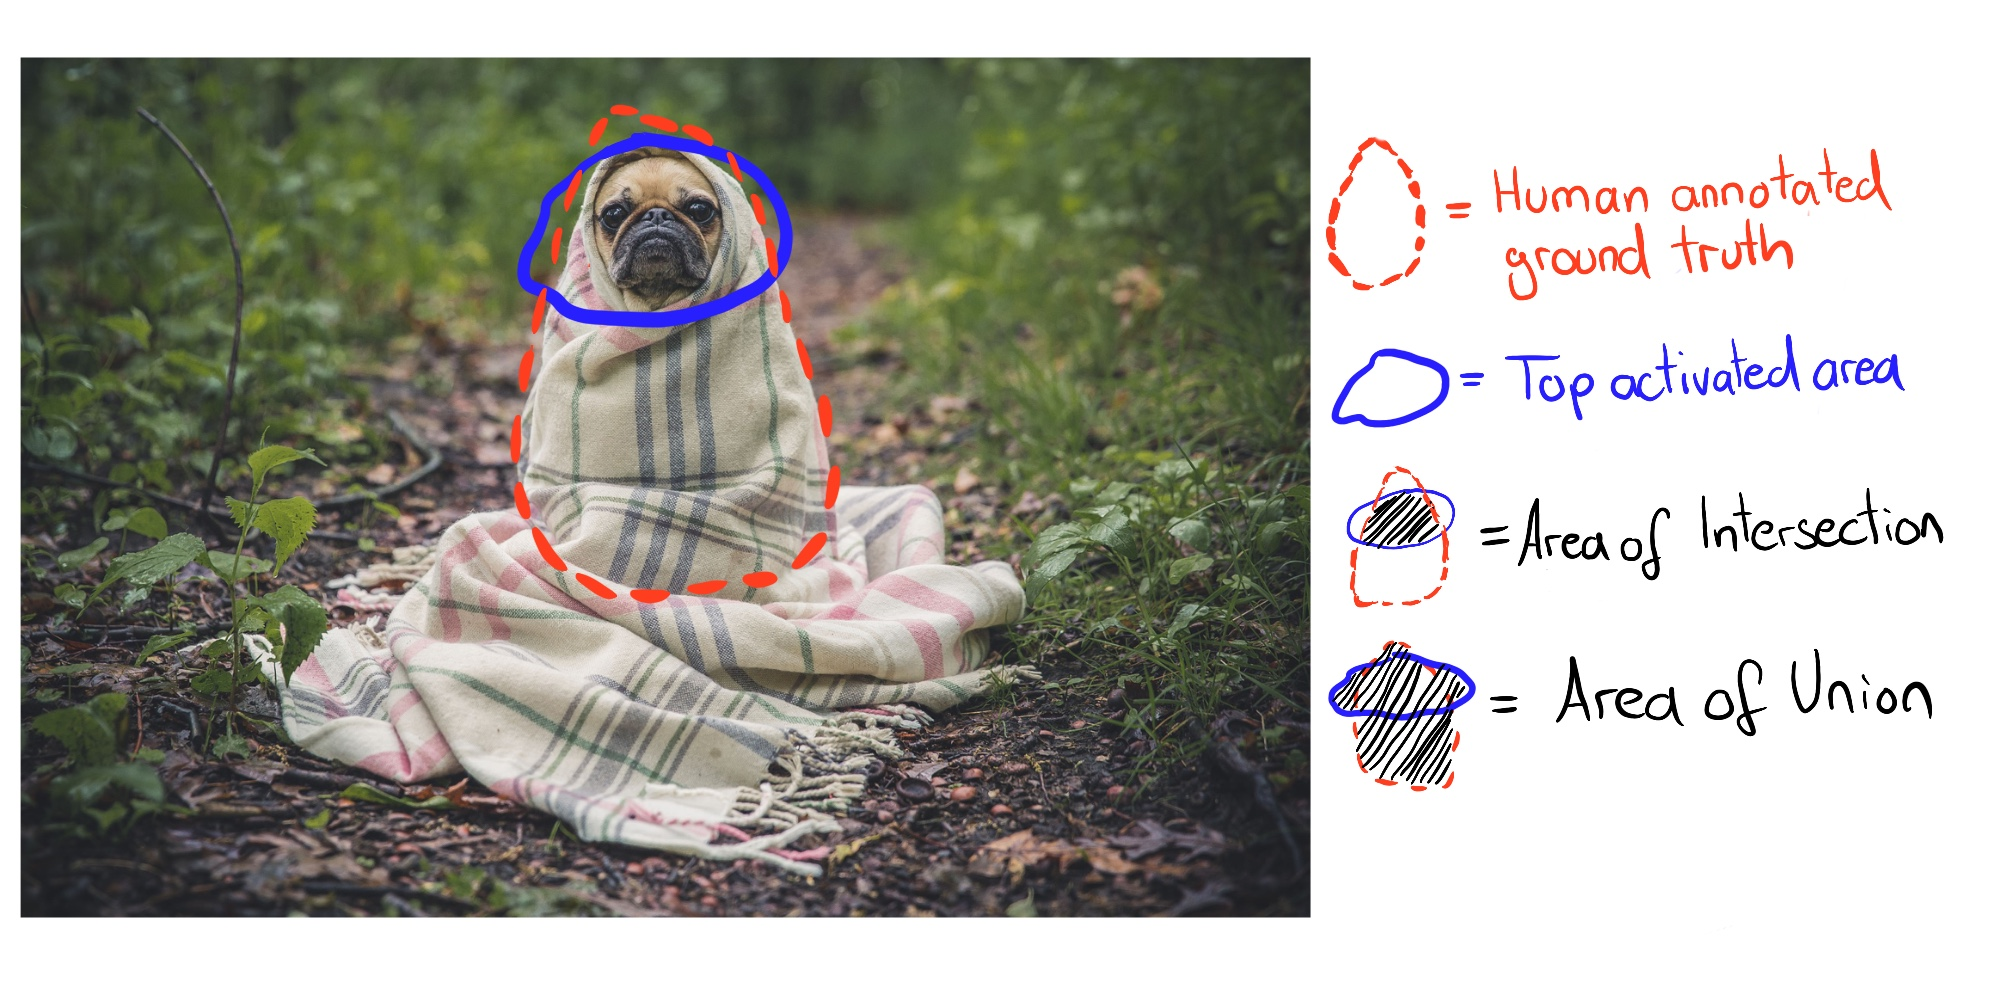
\includegraphics[scale=0.2]{images/dissection-dog-exemplary.jpg}
	\label{fig:7_7}
	\caption{IoU được tính toán bằng cách so sánh các phân vùng được gắn nhãn bởi người và các điểm ảnh có kích hoạt đứng đầu.}
\end{figure*}

Hình ảnh sau đây chỉ ra một thành phần phát hiện chó:

\begin{figure*}[h!]
	\centering
	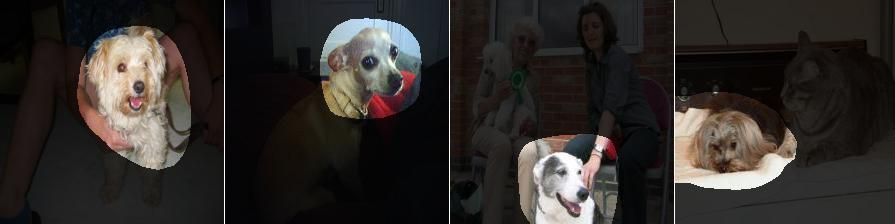
\includegraphics[scale=0.45]{images/dissection-dogs.jpeg}
	\label{fig:7_8}
	\caption{Mặt nạ kích hoạt cho inception\_4e kênh 750, kênh này phát hiện chó với IoU = 0.203.}
\end{figure*}

\subsubsection{Các thí nghiệm}

Tác giả của thuật toán phân tách mạng (Network Dissection) đã huấn luyện các kiến trúc mạng khác nhau (AlexNet, VGG, GoogleNet, ResNet) từ đầu (from scratches) trên các tập dữ liệu khác nhau (ImageNet, Places205, Places365). ImageNet chứa 1.6 triệu hình và 1000 lớp. Places205 và Places365 chứa 2.4 triệu và 1.6 triệu hình từ 205 và 365 khung cảnh khác nhau. Họ huấn luyện thêm AlexNet trên các bài toán huấn luyện tự giám sát (self-supervised training) ví dụ như dự đoán thứ tự khung hình video hoặc tô màu hình ảnh. Đối với các tùy chỉnh khác nhau, họ coi số bộ phát hiện khái niệm (duy nhất) là một thước đo của tính khả diễn giải. Đây là một số phát hiện:

- Các mạng phát hiện các khái niệm cấp độ thấp (màu sắc, kết cấu) tại những lớp thấp hơn và những khái niệm cao hơn (bộ phận, đối tượng) tại các lớp cao hơn. Chúng ta đã thấy được điều đó trong 7.1.1.

- Chuẩn hóa theo batch (Batch normalization) giảm thiểu số các bộ phát hiện khái niệm duy nhất.

- Nhiều thành phần trong mạng phát hiện cùng một khái niệm. Ví dụ, có 95 kênh phát hiện chó trong VGG được huấn luyện trên ImageNet khi sử dụng IoU > 0.04 (4 trong conv4\_3, 91 trong conv5\_3, xem trong \href{http://netdissect.csail.mit.edu/dissect/vgg16_imagenet/}{website dự án}).

- Việc tăng số kênh trong một lớp cũng đồng thời làm tăng số bộ phát hiện khái niệm.

- Các khởi tạo ngẫu nhiêu - random initializations (huấn luyện với các seed ngẫu nhiên khác nhau) cho kết quả hơi khác nhau về số lượng của các bộ phát hiện khái niệm.

- ResNet là một kiến trúc mạng với số bộ phát hiện duy nhất lớn nhất, tiếp theo là VGG, GoogleNet và AlexNet là cuối cùng.

- Số bộ phát hiện khái niệm duy nhất lớn nhất là được học từ Places365, tiếp theo là Places205 và ImageNet là cuối cùng.

- Số bộ phát hiện duy nhất tăng với số vòng lặp huấn luyện.


\begin{figure*}[h!]
	\centering
	\includegraphics[scale=0.3]{images/arch-compare.png}
	\label{fig:7_9}
	\caption{ResNet được huấn luyện trên Places365 có số phát hiện duy nhất cao nhất. AlexNet với các trọng số ngẫu nhiên có số bộ phát hiện duy nhất thấp nhất và được dùng làm tham chiếu. Hình ảnh gốc từ Bau \& Zhou et. al (2017).}
\end{figure*}

- Các mạng được huấn luyện trên các nhiệm vụ tự giám sát có các bộ phát hiện duy nhất ít hơn so với các mạng được huấn luyện trên các nhiệu vụ giám sát.

- Trong học truyền tải (transfer learning), khái niệm của một kênh có thể thay đổi. Ví dụ, một bộ phát hiện chó có thể trở thành bộ phát hiện thác nước. Điều này xảy ra trong một mô hình mà nó ban đầu được huấn luyện để phân loại các đối tượng và sau đó tinh chỉnh để phân loại khung cảnh.

- Trong một thí nghiệm, tác giả xem xét các kênh theo phương pháp mới (phương pháp xoay). Thí nghiệm được thực hiện với mạng VGG đã huấn luyến trên ImageNet. “Xoay” không có nghĩa rằng hình ảnh đã bị xoay. “Xoay” nghĩa là chúng ta lấy 256 kênh từ lớp conv5 và tính toán 256 kênh mới như là sự kết hợp tuyến tính của các kênh trước đó. Trong quá trình đó, các kênh là phi tách bạch (entangled). Sự xoay giảm bớt khả năng diễn giải, tức là số lượng kênh được điều chỉnh với một khái niệm giảm đi. Phép xoay được thiết kế để giữ cho hiệu suất của mô hình không đổi. Kết luận thứ nhất: Khả năng diễn giải của CNNs là phụ thuộc theo trục (axis-dependent). Điều này có nghĩa rằng việc kết hợp ngẫu nhiên các sẽ không có nhiều khả năng tạo ra các bộ phát hiện khái niệm duy nhất. Kết luận thứ hai: Khả năng diễn giải là độc lập với khả năng phân loại (discriminative power). Các kênh có thể được biến đổi với các phép biến đổi trực giao (orthogonal transformations) trong khi khả năng phân loại duy trì như cũ, nhưng khả năng diễn giải giảm đi.

\begin{figure*}[h!]
	\centering
	\includegraphics[scale=0.3]{images/rotation-dissect.png}
	\label{fig:7_10}
	\caption{Số các bộ phát hiện khái niệm duy nhất giảm đi khi 256 kênh của AlexNet conv5 (huấn luyện trên ImageNet) dần thay đổi trục bằng một phép biến đổi trực giao ngẫu nhiên. Hình ảnh gốc từ Bau $\&$ Zhou et. al (2017). Để hiểu rõ hơn, bạn có thể đọc thêm ở \href{http://openaccess.thecvf.com/content_cvpr_2017/papers/Bau_Network_Dissection_Quantifying_CVPR_2017_paper.pdf}{đây}.}
\end{figure*}

Các tác giả cũng đã sử dụng phân tách mạng cho GANs (Generative Adversarial Networks). Bạn có thể tìm thấy phân tách mạng cho GANs trên \href{https://gandissect.csail.mit.edu/}{website}.

\subsection{Ưu điểm}
Việc trực quan hóa đặc trưng cung cấp \textbf{cái nhìn sâu sắc độc đáo về hoạt động của các mạng nơ ron}, đặc biệt là bài toán nhận dạng hình ảnh. Với sự phức tạp và thiếu tường minh của các mạng nơ ron, việc trực quan hóa đặc trưng là một bước quan trọng trong việc phân tích và mô tả các mạng nơ ron. Thông qua việc trực quan hóa đặc trưng, chúng ta thấy rằng trong các lớp (layer) đầu tiên là các bộ phát hiện cạnh đơn giản cũng như kết cấu; trong khi các thành phần phát hiện khái niệm trừu tượng và đối tượng nằm ở các lớp cao hơn. Phân tách mạng cung cấp những hiểu biết và làm cho tính khả giải thích của các thành phần mạng có thể đo lường được.

Phân tách mạng cho phép chúng ta \textbf{tự động liên kết các thành phần với các khái niệm}, điểu này rõ ràng là rất hữu dụng. 

Trực quan hóa đặc trưng là một công cụ tuyệt vời để \textbf{thể hiện một cách đơn giản cách thức hoạt động của các mạng nơ ron}.

Với phân tách mạng, chúng ta cũng có thể \textbf{phát hiện các khái niệm ngoài các lớp (class) trong bài toán phân loại}. Nhưng chúng ta cần các bộ dữ liệu có chứa những hình ảnh với các khái niệm được gắn nhãn theo pixel như Broden.

Trực quan hóa đặc trưng có thể được \textbf{kết hợp với các phương pháp thành tố đặc trưng (feature attribution)}, nhằm giải thích pixel nào là quan trọng ứng với mỗi dự đoán. Sự kết hợp của cả hai phương pháp cho phép giải thích một dự đoán riêng lẻ cùng với trực quan hóa cục bộ các đặc trưng đã học có liên quan đến phân loại (xem thêm tại \href{https://distill.pub/2018/building-blocks/}{đây}).

\subsection{Nhược điểm}
\textbf{Nhiều hình ảnh từ trực quan hóa đặc trưng không có ý nghĩa}, chúng chứa một số đặc trưng trừu tượng mà ta không thể diễn giải bằng ngôn ngữ con người. Trong trường hợp này, hiển thị trực quan hóa đặc trưng cùng với dữ liệu huấn luyện có thể giúp ích. Ngoài ra, trực quan hóa vẫn không thể tiết lộ những gì mạng nơ-ron đã học mà chỉ hiển thị một cái gì đó có ``màu vàng''. Nhìn chung, kết quả vẫn là khá thô sơ. Ngay cả với phân tách mạng, một số kênh không được liên kết với khái niệm con người. Ví dụ: lớp conv5\_3 từ VGG được huấn luyện trên ImageNet có 193 kênh (trong số 512) không thể gắn với khái niệm của con người.

Có \textbf{quá nhiều thành phần để xem xét trong một mạng nơ-ron}, ngay cả khi ``chỉ'' xem xét các kích hoạt của kênh kênh. Đối với Inception V1, đã có hơn 5000 kênh từ 9 lớp chập. Nếu ta hiển thị cả kích hoạt âm và một vài hình ảnh từ dữ liệu huấn luyện cho kích hoạt tối đa hoặc tối thiểu (giả sử 4 âm, 4 dương), thì ta phải hiển thị hơn 50.000 hình ảnh. Ít nhất chúng ta biết - nhờ phân tách mạng - chúng ta đã có một chút cơ sở cho việc phân tích.

\textbf{Ảo tưởng về tính khả giải thích?} Các trực quan hóa đặc trưng có thể truyền tải ảo ảnh rằng chúng ta hiểu mạng nơ-ron đang làm gì. Nhưng chúng ta có thực sự hiểu những gì đang xảy ra trong mạng nơ-ron? Ngay cả khi chúng ta nhìn vào hàng trăm hoặc hàng ngàn hình ảnh trực quan, chúng ta không thể hiểu được mạng nơ ron. Các kênh tương tác theo một cách phức tạp, kích hoạt tích cực và tiêu cực không liên quan đến nhau, nhiều nơ-ron có thể học các đặc trưng rất giống nhau và đối với nhiều đặc trưng chúng ta không có khái niệm tương đương với con người. Chúng ta không nên tin rằng chúng ta hoàn toàn hiểu mạng nơ ron chỉ vì chúng ta tin rằng chúng ta đã thấy rằng tế bào nơ ron 349 ở lớp 7 được kích hoạt bởi hoa daisy. Phân tích mạng cho thấy các kiến trúc như ResNet hoặc Inception có các thành phần mà phản ứng với các khái niệm nhất định. Nhưng IoU không phải là một thước đo hoàn chỉnh và thường thì sẽ có nhiều thành phần phản ứng với cùng một khái niệm và một số không phản ứng với khái niệm nào cả. Các kênh không hoàn toàn tách rời và chúng ta không thể giải thích chúng một cách cô lập.

Đối với phân tách mạng, \textbf{bạn cần các bộ dữ liệu được gắn nhãn ở cấp độ pixel} với các khái niệm. Các bộ dữ liệu này mất rất nhiều nỗ lực để thu thập, vì mỗi pixel cần được dán nhãn, thường hoạt động bằng cách vẽ các phân đoạn xung quanh các đối tượng trên hình ảnh.

Phân tách mạng chỉ điều chỉnh các khái niệm của con người với các kích hoạt dương chứ không phải với các kích hoạt âm của các kênh. Như các trực quan hóa đặc trưng  cho thấy, kích hoạt âm dường như cũng được liên kết với các khái niệm.

\subsection{Phần mềm và tài liệu khác}
Có một bộ mã nguồn mở của trực quan hóa đặc trưng được gọi là \href{https://github.com/tensorflow/lucid}{Lucid}. Bạn có thể dùng thử trong trình duyệt của mình bằng cách sử dụng các liên kết notebook được cung cấp trên trang Lucid Github. Không có phần mềm bổ sung được yêu cầu. Các chương trình khác bao gồm \href{https://github.com/InFoCusp/tf_cnnvis}{tf\_cnnvis} cho TensorFlow, \href{https://github.com/jacobgil/keras-filter-visualization}{Bộ lọc Keras} cho Keras và \href{https://github.com/yosinski/deep-visualization-toolbox}{DeepVis} cho Caffe.

Network Dissection có một \href{http://netdissect.csail.mit.edu/}{trang web dự án} tuyệt vời. Bên cạnh bài báo, trang web lưu trữ các tài liệu bổ sung như mã code, dữ liệu và trực quan hóa của các mặt nạ kích hoạt.
